%\documentclass[compress]{beamer}
\documentclass[8pt,xcolor=dvipnames]{beamer}

%-----------------------------------------------------------
% PACKAGES

%\usepackage[latin1]{inputenc}
\mode<presentation>

%\usepackage[T1]{fontenc}  
%\usetheme{Warsaw}
\usetheme{Frankfurt}
\definecolor{maroon}{RGB}{80, 0.0, 0.0}
\usecolortheme[named=maroon]{structure}
%\setbeamercolor{block title}{bg=red!30,fg=black}

\usepackage{graphicx}
%\usepackage[section]{placeins} % force � mettre l'image o� on veut
%\usepackage{float} %utiliser H pour forcer � mettre l'image o� on veut
\usepackage{lscape} %utilisation du mode paysage
%\usepackage{pslatex}
\usepackage{url}
\usepackage{subfigure}

\usepackage{graphicx}
\usepackage{tabls}
\usepackage{afterpage}

\usepackage{ocgx2}
\usepackage[]{media9}
%\usepackage{multimedia}

\usepackage{amsthm}
\usepackage{amssymb}
\usepackage{amsmath}
\usepackage{amsfonts}
\usepackage{amstext}
\usepackage{amsbsy}
\usepackage{mathbbol} 
\usepackage{mathrsfs}

\usepackage{epsfig}
%\usepackage{epsfig}
%\usepackage{cites}
\usepackage{epsf}
\usepackage{array}
\usepackage{color}
\usepackage{pdfpages}
\usepackage{cancel}

\usepackage{tikz}
\usepackage{colortbl}
%\usepackage{booktabs}

%-----------------------------------------------------------
% NEW  DEFINITIONS
%
%=================================================================================================
% new commands
% +++++++++++++++++++++++++++++++++++++++++++++++++++++++++++++++++++++++++++++++++++++++++++++++++
\newcommand{\nc}{\newcommand}
%
% Ways of grouping things
%
\newcommand{\bracket}[1]{\left[ #1 \right]}
\newcommand{\bracet}[1]{\left\{ #1 \right\}}
\newcommand{\fn}[1]{\left( #1 \right)}
\newcommand{\ave}[1]{\left\langle #1 \right\rangle}
%
% Derivative forms
% 
\newcommand{\dx}[1]{\,d#1}
\newcommand{\dxdy}[2]{\frac{\partial #1}{\partial #2}}
\newcommand{\dxdt}[1]{\frac{\partial #1}{\partial t}}
\newcommand{\dxdz}[1]{\frac{\partial #1}{\partial z}}
\newcommand{\dfdt}[1]{\frac{\partial}{\partial t} \fn{#1}}
\newcommand{\dfdz}[1]{\frac{\partial}{\partial z} \fn{#1}}
\newcommand{\ddt}[1]{\frac{\partial}{\partial t} #1}
\newcommand{\ddz}[1]{\frac{\partial}{\partial z} #1}
\newcommand{\dd}[2]{\frac{\partial}{\partial #1} #2}
\newcommand{\ddx}[1]{\frac{\partial}{\partial x} #1}
\newcommand{\ddy}[1]{\frac{\partial}{\partial y} #1}
%
% Vector forms
%
%\renewcommand{\vec}[1]{\ensuremath{\stackrel{\rightarrow}{#1}}}
%\renewcommand{\div}{\ensuremath{\vec{\nabla} \cdot}}
%\newcommand{\grad}{\ensuremath{\vec{\nabla}}}

\renewcommand{\div}{\vec{\nabla}\! \cdot \!}
\newcommand{\grad}{\vec{\nabla}}
\newcommand{\oa}[1]{\fn{\frac{1}{3}\hat{\Omega}\!\cdot\!\overrightarrow{A_{#1}}}}

%
% Equation beginnings and endings
%
\newcommand{\bea}{\begin{eqnarray}}
\newcommand{\eea}{\end{eqnarray}}
\newcommand{\be}{\begin{equation*}}
\newcommand{\ee}{\end{equation*}}
\newcommand{\beas}{\begin{eqnarray*}}
\newcommand{\eeas}{\end{eqnarray*}}
\newcommand{\bdm}{\begin{displaymath}}
\newcommand{\edm}{\end{displaymath}}
%
% Equation punctuation
% 
\newcommand{\pec}{\hspace{0.25in},}
\newcommand{\pep}{\hspace{0.25in}.}
\newcommand{\pev}{\hspace{0.25in}}
%
% Equation labels and references, figure references, table references
% 
\newcommand{\LEQ}[1]{\label{eq:#1}}
\newcommand{\EQ}[1]{Eq.~(\ref{eq:#1})}
\newcommand{\EQS}[1]{Eqs.~(\ref{eq:#1})}
\newcommand{\REQ}[1]{\ref{eq:#1}}
\newcommand{\LFI}[1]{\label{fi:#1}}
\newcommand{\FI}[1]{Fig.~\ref{fi:#1}}
\newcommand{\RFI}[1]{\ref{fi:#1}}
\newcommand{\LTA}[1]{\label{ta:#1}}
\newcommand{\TA}[1]{Table~\ref{ta:#1}}
\newcommand{\RTA}[1]{\ref{ta:#1}}

%
% List beginnings and endings
% 
\newcommand{\bl}{\bss\begin{itemize}}
\newcommand{\el}{\vspace{-.5\baselineskip}\end{itemize}\ess}
\newcommand{\benu}{\bss\begin{enumerate}}
\newcommand{\eenu}{\vspace{-.5\baselineskip}\end{enumerate}\ess}
%
% Figure and table beginnings and endings
% 
\newcommand{\bfg}{\begin{figure}}
\newcommand{\efg}{\end{figure}}
\newcommand{\bt}{\begin{table}}
\newcommand{\et}{\end{table}}
%
% Tabular and center beginnings and endings
% 
\newcommand{\bc}{\begin{center}}
\newcommand{\ec}{\end{center}}
\newcommand{\btb}{\begin{center}\begin{tabular}}
\newcommand{\etb}{\end{tabular}\end{center}}
%
% Single space command
% 
%\newcommand{\bss}{\begin{singlespace}}
%\newcommand{\ess}{\end{singlespace}}
\newcommand{\bss}{\singlespacing}
\newcommand{\ess}{\doublespacing}
%
%---New environment "arbspace". (modeled after singlespace environment
%                                in Doublespace.sty)
%   The baselinestretch only takes effect at a size change, so do one.
% 
\def\arbspace#1{\def\baselinestretch{#1}\@normalsize}
\def\endarbspace{}
\newcommand{\bas}{\begin{arbspace}}
\newcommand{\eas}{\end{arbspace}}
%
% An explanation for a function
%
\newcommand{\explain}[1]{\mbox{\hspace{2em} #1}}
%
% Quick commands for symbols
%  
\newcommand{\half}{\frac{1}{2}}
\newcommand{\third}{\frac{1}{3}}
\newcommand{\twothird}{\frac{2}{3}}
\newcommand{\fourth}{\frac{1}{4}}
\newcommand{\mdot}{\dot{m}}
\newcommand{\ten}[1]{\times 10^{#1}\,}
\newcommand{\cL}{{\cal L}}
\newcommand{\cD}{{\cal D}}
\newcommand{\cF}{{\cal F}}
\newcommand{\cE}{{\cal E}}
\renewcommand{\Re}{\mbox{Re}}
\newcommand{\Ma}{\mbox{Ma}}
%
% Inclusion of Graphics Data
%
%\input{psfig}
%\psfiginit
%
% More Quick Commands
% 
\newcommand{\bi}{\begin{itemize}}
\newcommand{\ei}{\end{itemize}}
\newcommand{\ben}{\begin{enumerate}}
\newcommand{\een}{\end{enumerate}}
\newcommand{\dxi}{\Delta x_i}
\newcommand{\dyj}{\Delta y_j}
\newcommand{\ts}[1]{\textstyle #1}


\newcommand{\bu}{\boldsymbol{u}}
\newcommand{\ber}{\boldsymbol{e}}
\newcommand{\br}{\boldsymbol{r}} 
\newcommand{\bo}{\boldsymbol{\Omega}}

\newcommand{\bn}{\boldsymbol{\nabla}}

% DGFEM commands
\newcommand{\jmp}[1]{[\![#1]\!]}                     % jump
\newcommand{\mvl}[1]{\{\!\!\{#1\}\!\!\}}             % mean value


\newcommand{\boxedeqn}[1]{%
  \[\fbox{%
      \addtolength{\linewidth}{-2\fboxsep}%
      \addtolength{\linewidth}{-2\fboxrule}%
      \begin{minipage}{\linewidth}%
      \begin{equation}#1\end{equation}%
      \end{minipage}%
    }\]%
}
\newcommand{\mboxed}[1]{\boxed{\phantom{#1}}}
\newcommand{\ud}{\,\mathrm{d}}

% keff
\newcommand{\keff}{\ensuremath{k_{\textit{eff}}}}

% margin par
\newcommand{\mt}[1]{\marginpar{ {\footnotesize #1} }}

% shortcut for aposterio in italics
\newcommand{\apost}{\textit{a posteriori\xspace}}
\newcommand{\Apost}{\textit{A posteriori}\xspace}

% shortcut for multi-group
\newcommand{\mg}{multigroup\xspace}
\newcommand{\Mg}{Multigroup\xspace}
\newcommand{\ho}{higher-order\xspace}
\newcommand{\Ho}{Higher-order\xspace}
\newcommand{\HO}{Higher-Order\xspace}
\newcommand{\HObig}{HIGHER-ORDER\xspace}
\newcommand{\Mgbig}{MULTIGROUP\xspace}

% shortcut for domain notation
\newcommand{\D}{\mathcal{D}}

% shortcut for xuthus
\newcommand{\psc}[1]{{\sc {#1}}}
\newcommand{\xuthus}{\psc{xuthus}\xspace}

% vector shortcuts
\newcommand{\vo}{\vec{\Omega}}
\newcommand{\vr}{\vec{r}}
\newcommand{\vn}{\vec{n}}
\newcommand{\vnk}{\vec{\mathbf{n}}}

% extra space
\newcommand{\qq}{\quad\quad}

% sign function
\DeclareMathOperator{\sgn}{sgn}


\newcommand{\ensuretext}[1]{\ensuremath{\text{#1}}}

% common reference commands
\newcommand{\eqt}[1]{Eq.~(\ref{#1})}                     % equation
\newcommand{\fig}[1]{Fig.~\ref{#1}}                      % figure
\newcommand{\tbl}[1]{Table~\ref{#1}}                     % table



\newcommand{\rhs}{right-hand-side\xspace}
\newcommand{\clearemptydoublepage}{\newpage{\pagestyle{empty}\cleardoublepage}}


\newcommand{\bs}[1]{\mathbf{#1}}
\renewcommand{\bs}[1]{\vec{#1}}
%\newcommand{\dd}{\mathrm{d}}
\newcommand{\norm}[1]{\left\lVert#1\right\rVert_{L^2}}
\renewcommand{\Re}{\textrm{Re}}
\newcommand{\Pe}{\textrm{P\'e}}
\renewcommand{\Pr}{\textrm{Pr}}

\newcommand{\resi}{R_e}
%\newcommand{\resinew}{\tilde{D}_e}
\newcommand{\resinew}{\widetilde{\resi}}
\newcommand{\matder}[1]{\frac{\textrm{D} #1}{\textrm{D} t}}

\newcommand{\divv}[1]{\vec{\nabla}^{#1}\! \cdot \!}
\newcommand{\gradd}[1]{\vec{\nabla}^{#1}}

\definecolor{britishracinggreen}{rgb}{0.0, 0.26, 0.15}
\newcommand{\tcr}[1]{\textcolor{red}{#1}}
\newcommand{\tcb}[1]{\textcolor{blue}{#1}}
\newcommand{\tcm}[1]{\textcolor{magenta}{#1}}
\newcommand{\tcp}[1]{\textcolor{violet}{#1}}
\newcommand{\tcg}[1]{\textcolor{britishracinggreen}{#1}}

\renewcommand{\L}{\mathbf{L}}
\renewcommand{\S}{\mathbf{\Sigma}}
\newcommand{\M}{\mathbf{M}}
\renewcommand{\D}{\mathbf{D}}

% tikz stuff
\usetikzlibrary{shapes,arrows,positioning}
\pgfdeclarelayer{background}
\pgfdeclarelayer{foreground}
\pgfsetlayers{background,main,foreground}
\tikzstyle{redblock}=[rectangle, draw, align=center, top color=red!25, bottom color=red!75,  minimum width=10mm, minimum height=10mm,]
\tikzstyle{blueblock}=[rectangle,draw, align=center, top color=blue!25, bottom color=blue!75,  minimum width=10mm, minimum height=10mm]
\tikzstyle{purpleblock}=[rectangle,  draw, align=center, top color=purple!25, bottom color=purple!75, minimum width=10mm, minimum height=10mm]
\tikzstyle{orangeblock}=[rectangle, draw, align=center, top color=orange!25, bottom color=orange!75,  minimum width=10mm, minimum height=10mm]
\tikzstyle{greendiamond}=[diamond, draw, align=center, top color=green!25, bottom color=green!75,  minimum width=8mm, aspect=2]

%=================================================================================================

%============================================================

%style et couleur
%\usetheme{Frankfurt}
\date{\today}

%\addtobeamertemplate{footline}{\hfill\insertframenumber/\inserttotalframenumber\hspace{2em}\null}

\setbeamertemplate{footline}{
\leavevmode%
%\hbox{\hspace*{-0.06cm}
\begin{beamercolorbox}[wd=.5\paperwidth,ht=3.25ex,dp=1ex,center]{author in head/foot}%
	\usebeamerfont{author in head/foot}\insertshortauthor%~~(\insertshortinstitute)
\end{beamercolorbox}%
\begin{beamercolorbox}[wd=.25\paperwidth,ht=3.25ex,dp=1ex,center]{section in head/foot}%
	\usebeamerfont{section in head/foot} IQS November 2016 % \insertshorttitle
\end{beamercolorbox}%
\begin{beamercolorbox}[wd=.25\paperwidth,ht=3.25ex,dp=1ex,left]{section in head/foot}%
	\usebeamerfont{section in head/foot}\insertshortdate{}\hspace*{2em}
	\insertframenumber{} / \inserttotalframenumber %\hspace*{2ex}
\end{beamercolorbox}}%
%\vskip0pt%
%}

\beamertemplatetransparentcovered

\urldef{\ragusa}\url{jean.ragusa@tamu.edu}
\urldef{\prince}\url{zachmprince@tamu.edu}

\title{TREAT Support: Improved Quasi-Static Method}

\author{Zachary M. Prince, Jean C. Ragusa}
\institute{Department of Nuclear Engineering, Texas A\&M University, College Station, TX}

\logo{
\includegraphics[height=0.8cm]{figures/inl-logo.png}
      \includegraphics[height=0.8cm]{figures/TAM-logo.png}}

%%%%%%%%%%%%%%%%%%%%%%%%%%%%%%%%%%%%%%%%%%%%%%%%%%%%%%%%%%%%%%%%%%%%

%%%%%%%%%%%%%%%%%%%%%%%%%%%%%%%%%%%%%%%%%%%%%%%%%%%%%%%%%%%%%%%%%%%%
%%%%%%%%%%%%%%%%%%%%%%%%%%%%%%%%%%%%%%%%%%%%%%%%%%%%%%%%%%%%%%%%%%%%
\begin{document}
%%%%%%%%%%%%%%%%%%%%%%%%%%%%%%%%%%%%%%%%%%%%%%%%%%%%%%%%%%%%%%%%%%%%
%%%%%%%%%%%%%%%%%%%%%%%%%%%%%%%%%%%%%%%%%%%%%%%%%%%%%%%%%%%%%%%%%%%%

%-------------------------------------------------------------------
\begin{frame}
%\vspace{-1.5cm}
	\begin{figure}[t]
		\centering
			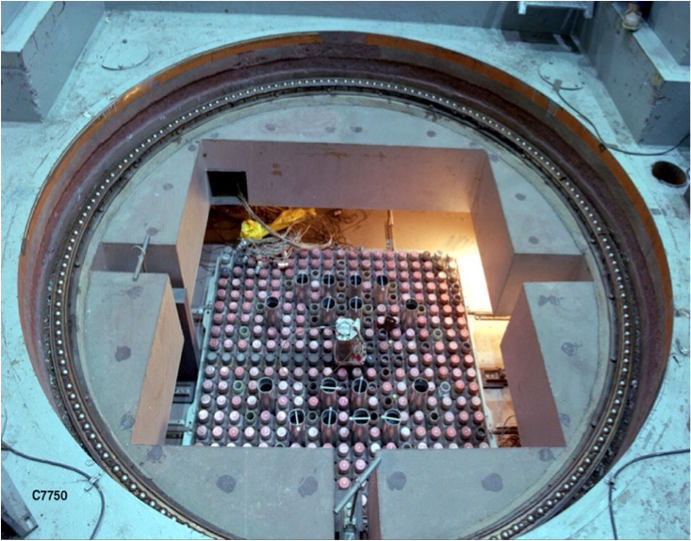
\includegraphics[width=.45\textwidth]{figures/Treat_core_view.png}
	\end{figure}
\vspace{-0.5cm}
\titlepage
\vspace{-0.5cm}
\small{email: {\prince} }

\end{frame}
%-------------------------------------------------------------------

%-------------------------------------------------------------------
\begin{frame}
	\frametitle{Outline}
	\tableofcontents 
\end{frame}
%-------------------------------------------------------------------

%%%%%%%%%%%%%%%%%%%%%%%%%%%%%%%%%%%%%%%%%%%%%%%%%%%%%%%%%%%%%%%%%%%%
%%%%%%%%%%%%%%%%%%%%%%%%%%%%%%%%%%%%%%%%%%%%%%%%%%%%%%%%%%%%%%%%%%%%
\section{IQS Review}
%%%%%%%%%%%%%%%%%%%%%%%%%%%%%%%%%%%%%%%%%%%%%%%%%%%%%%%%%%%%%%%%%%%%
%%%%%%%%%%%%%%%%%%%%%%%%%%%%%%%%%%%%%%%%%%%%%%%%%%%%%%%%%%%%%%%%%%%%

%%%%%%%%%%%%%%%%%%%%%%%%%%%%%%%%%%%%%%%%%%%%%%%%%%%%%%%%%%%%%%%%%%%%
\subsection{Equations}
%%%%%%%%%%%%%%%%%%%%%%%%%%%%%%%%%%%%%%%%%%%%%%%%%%%%%%%%%%%%%%%%%%%%


%-------------------------------------------------------------------
\begin{frame}{IQS Traditional}

\vspace{-3mm}

\begin{block}{Factorization}
\begin{equation*}
\phi^g(\vec{r},t) = \tcr{p(t)} \tcb{\varphi^g(\vec{r},t)}
\end{equation*}
\end{block}

\vspace{-2mm}

\begin{block}{Shape equations}
\begin{align*}
\frac{1}{v^g} \frac{\partial \tcb{\varphi^g} }{\partial t} =& \frac{\chi_p^g}{\keff} \sum_{g'=1}^G (1-\beta) \nu^{g'} \Sigma_f^{g'} \tcb{\varphi^{g'}} -  \left( -\div D^g \grad  + \Sigma_r^g + \tcr{\frac{1}{v^g}}\tcr{\frac{1}{p}}\tcr{\frac{dp}{dt}}\right) \tcb{\varphi^g}  \nonumber \\
&  + \sum_{g'\neq g}^G\Sigma_s^{g'\to g} \tcb{\varphi^{g'}}  + \tcr{\frac{1}{p}}\sum_{i=1}^I\chi_{d,i}^g\lambda_i C_i \ , \quad 1 \le g \le G 
\end{align*}
\begin{equation*}
\frac{dC_i}{dt} = \tcr{p}\sum_{g=1}^G \nu_{d,i} \Sigma_f^g \tcb{\varphi^{g}} - \lambda_iC_i , \quad 1 \le i \le I
\end{equation*}
%\be
%\frac{dC_i}{dt} = \frac{\beta_i}{k_{eff}}\sum_{g=1}^G\nu^{g} \Sigma_f^g \tcr{p} \varphi^{g} - \lambda_i C_i \ , \quad 1 \le i \le I 
%\ee
\end{block}

\vspace{-2mm}

\begin{block}{PRKE}
\[
\frac{d\tcr{p}}{dt}=\left[\frac{\rho-\bar{\beta}}{\Lambda}\right]\tcr{p}+\sum_{i=1}^I\bar{\lambda}_i\xi_i
\]
\[
\frac{d\xi_i}{dt}=\frac{\bar{\beta}_i}{\Lambda}\tcr{p} - \bar{\lambda}_i\xi_i \quad 1 \le i \le I 
\]
\end{block}
%\vspace{-3mm}

\end{frame}
%-------------------------------------------------------------------

%-------------------------------------------------------------------
\begin{frame}{IQS Predictor-Corrector}

\vspace{-3mm}

\begin{block}{Predicted Flux $\rightarrow$ Corrected Flux}
IQS P-C linearizes the system and avoids iterations on the \tcb{shape}: 
\ben
\item Evaluate multigroup diffusion equation to get predicted flux $\phi_{n+1}^{g,\tcr{pred}}$
\item Scale predicted flux to obtain \tcb{shape}:
\[
\tcb{\varphi^{g}_{n+1}} = \phi_{n+1}^{g,\tcr{pred}} \frac{\sum_{g=1}^G\left(\phi^{*g},\frac{1}{v^g}\phi ^g_{0}\right)}{\sum_{g=1}^G \left(\phi^{*g},\frac{1}{v^g}\phi_{n+1}^{g,\tcr{pred}}\right)} = \phi_{n+1}^{g,\tcr{pred}} \frac{\tcp{K_0}}{\tcp{K_{n+1}}}
\]
\item Compute PRKE parameters at $t_{n+1}$
\item Evaluate PRKE along micro step using interpolated parameters to obtain $\tcr{p_{n+1}}$
\item Scale $\tcb{\varphi^{g}_{n+1}}$ to obtain corrected flux:
\[
\phi_{n+1}^{g,\tcr{corr}} = \tcr{p_{n+1}} \times \tcb{\varphi^{g}_{n+1}}
\]
\een
\end{block}

\end{frame}
%-------------------------------------------------------------------

%%%%%%%%%%%%%%%%%%%%%%%%%%%%%%%%%%%%%%%%%%%%%%%%%%%%%%%%%%%%%%%%%%%%
\subsection{Process}
%%%%%%%%%%%%%%%%%%%%%%%%%%%%%%%%%%%%%%%%%%%%%%%%%%%%%%%%%%%%%%%%%%%%


%-------------------------------------------------------------------
\begin{frame}{Solution Process}

\begin{block}{Factorization leads to a nonlinear system}
The \tcr{amplitude} and \tcb{shape} equations form a system of nonlinear coupled equations: 
\ben
\item the coefficients appearing in the \tcr{PRKE}'s depend upon the \tcb{shape} solution,
\item the \tcb{shape} equation has a kernel dependent on \tcr{amplitude} and its derivative,  
%\item the delayed neutron source term is scaled by the amplitude.
\een
\end{block}

\begin{block}{Time scales and IQS method solution process}
Because solving for the \tcb{shape} can be expensive, especially in two or three dimensions, it is attractive to make the assumption that the \tcb{shape} is weakly time-dependent so the \tcb{shape} can be computed after a multitude of \tcr{PRKE} calculations:
%

\begin{figure}[h]
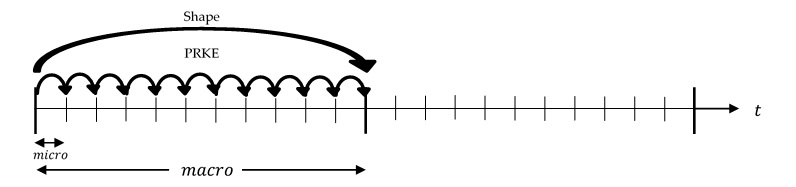
\includegraphics[width=\linewidth]{figures/IQS_visualization.jpg}
%\caption{IQS method solution process}
\label{fig:IQS}
\end{figure}

\end{block}
\end{frame}
%-------------------------------------------------------------------


\subsection{Transient-15}

%-------------------------------------------------------------------
\begin{frame}{TREAT: Transient-15}

%\begin{block}
\begin{figure}[h]
\centering
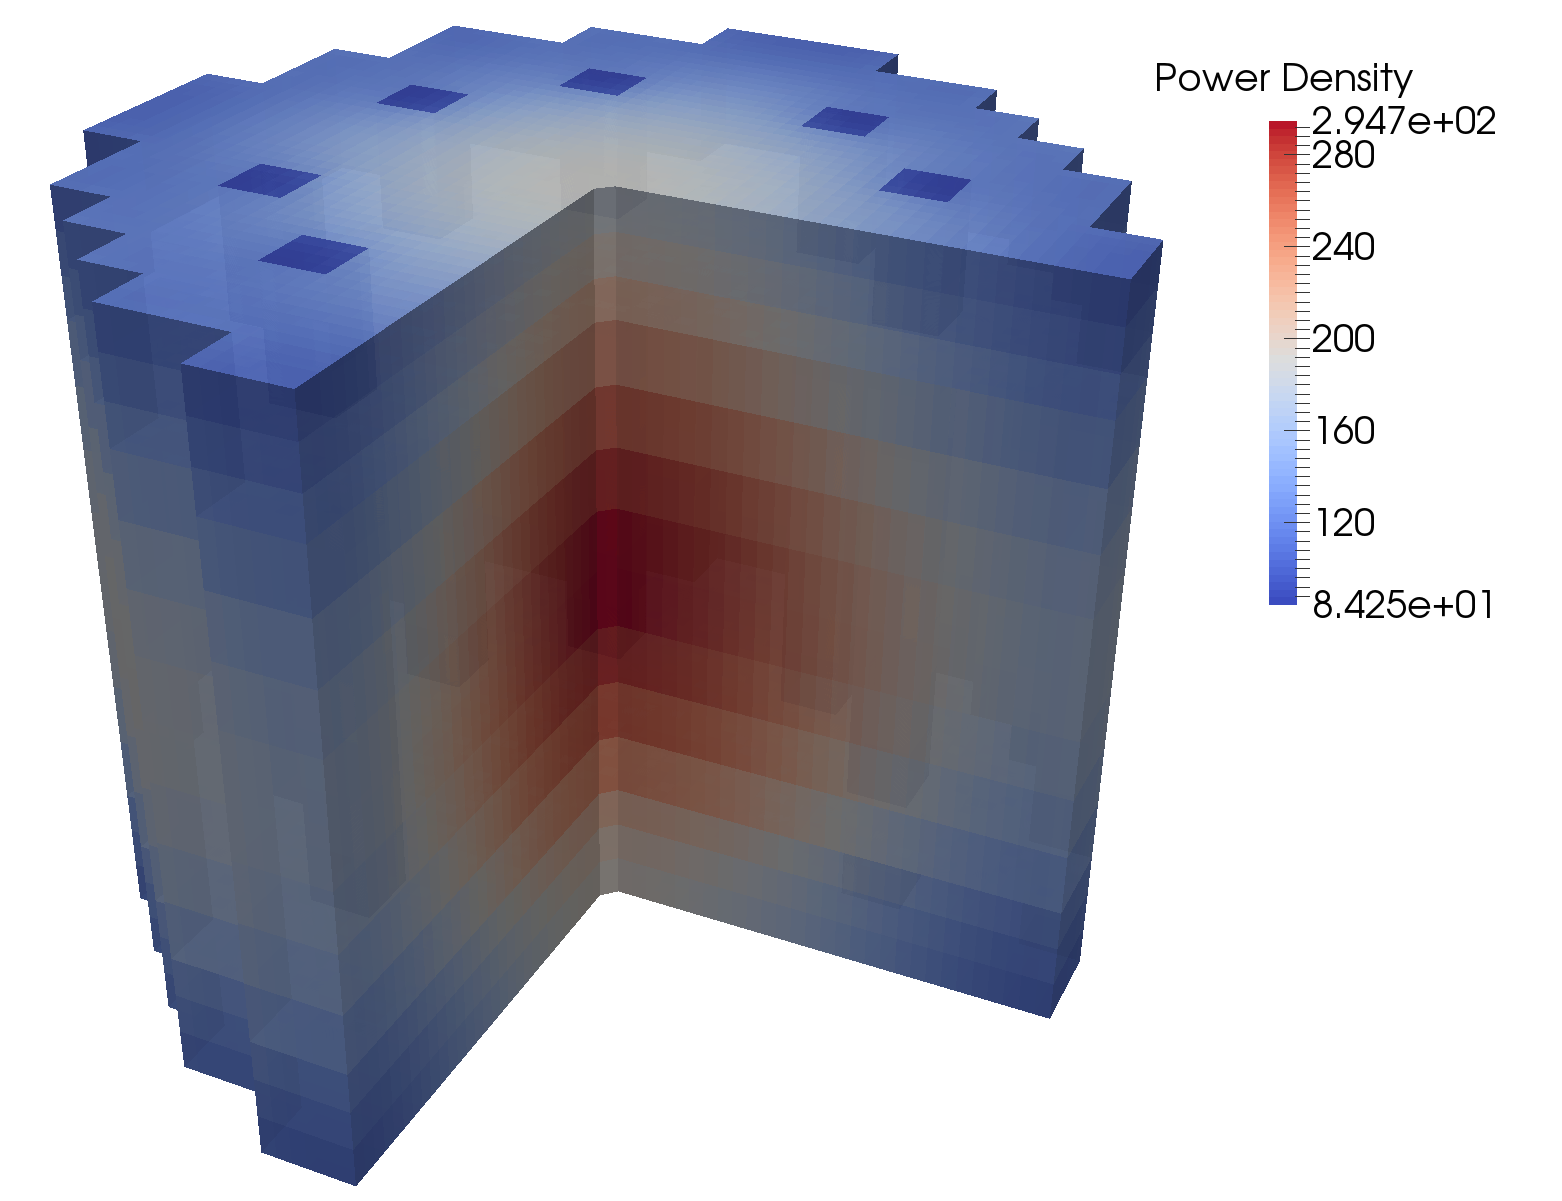
\includegraphics[height=0.9\textheight]{figures/Tran15_core2.png}
\end{figure}
%\end{block}

\end{frame}
%-------------------------------------------------------------------

%-------------------------------------------------------------------
\begin{frame}{Tran15 Results}

\begin{columns}

\column{.6\textwidth}
\begin{figure}
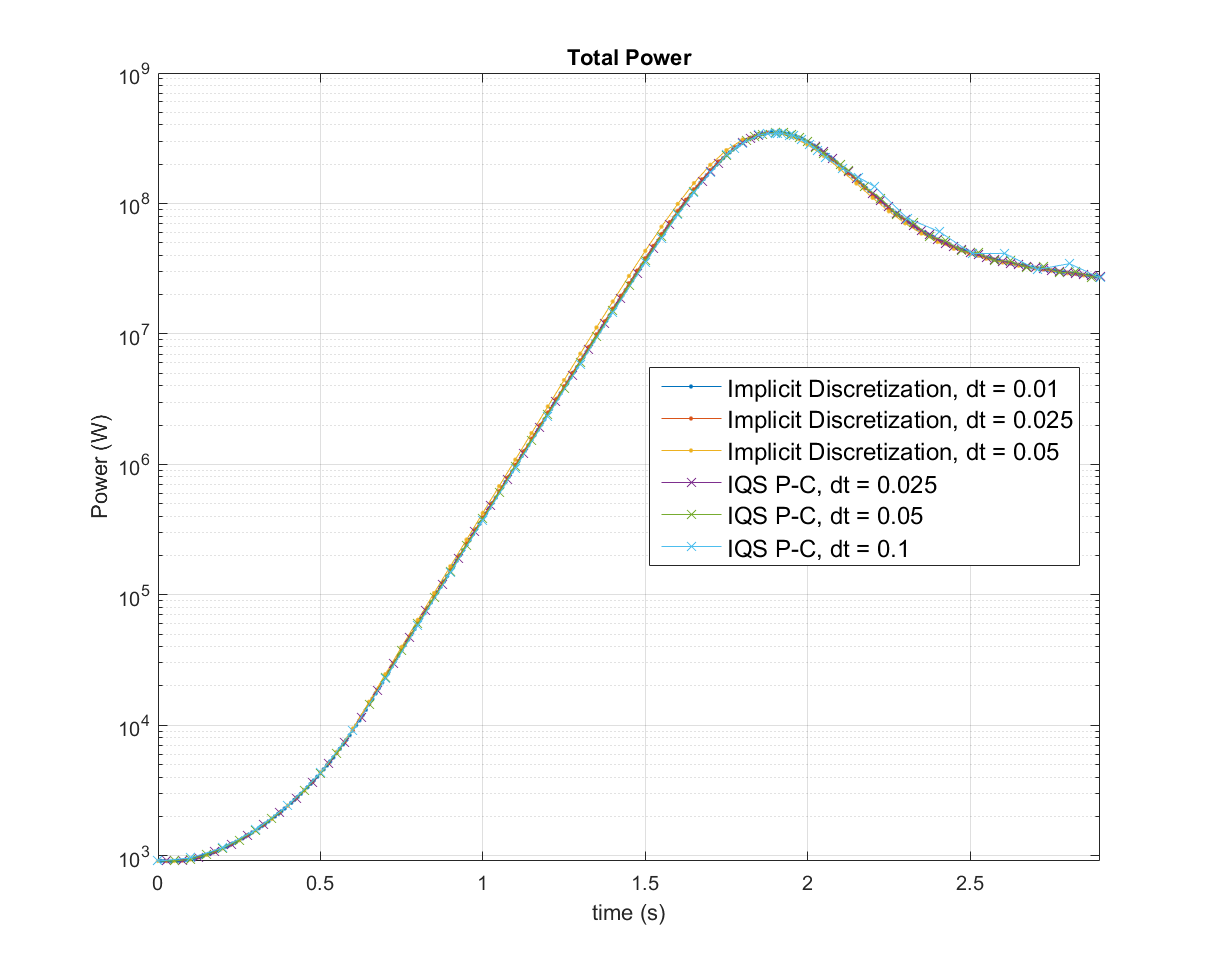
\includegraphics[width=\linewidth]{figures/Tran15_1.png}
\caption{Tran15 Power Profile}
\end{figure}

\column{.6\textwidth}
\begin{figure}
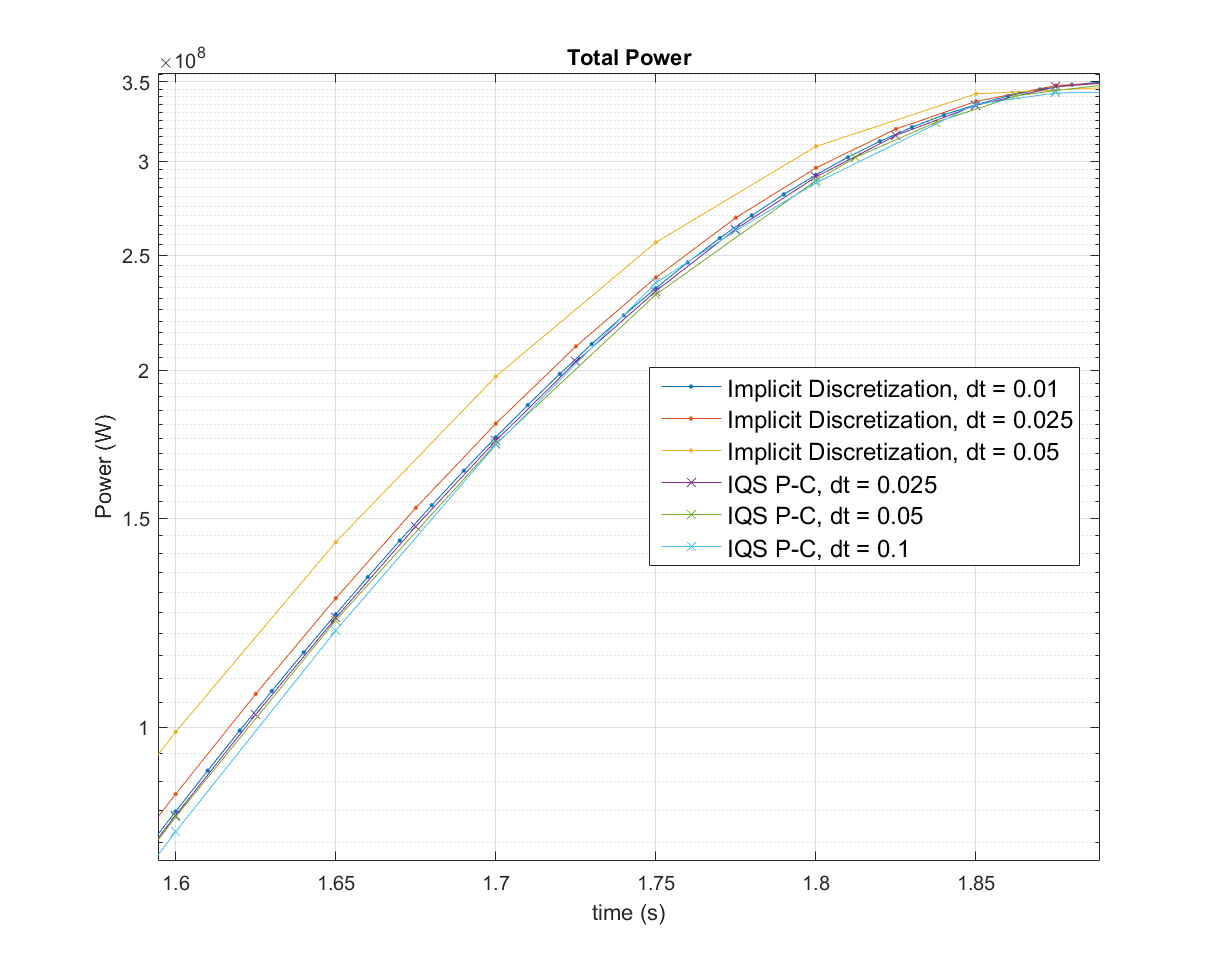
\includegraphics[width=\linewidth]{figures/Tran15_2.png}
\caption{Tran15 Peak Power Profile}
\end{figure}

\end{columns}

\end{frame}
%-------------------------------------------------------------------

\subsection{M8CAL}

%-------------------------------------------------------------------
\begin{frame}{TREAT: M8CAL}

\begin{columns}

\column{.6\textwidth}
\begin{figure}
\caption{M8CAL Power Profile}
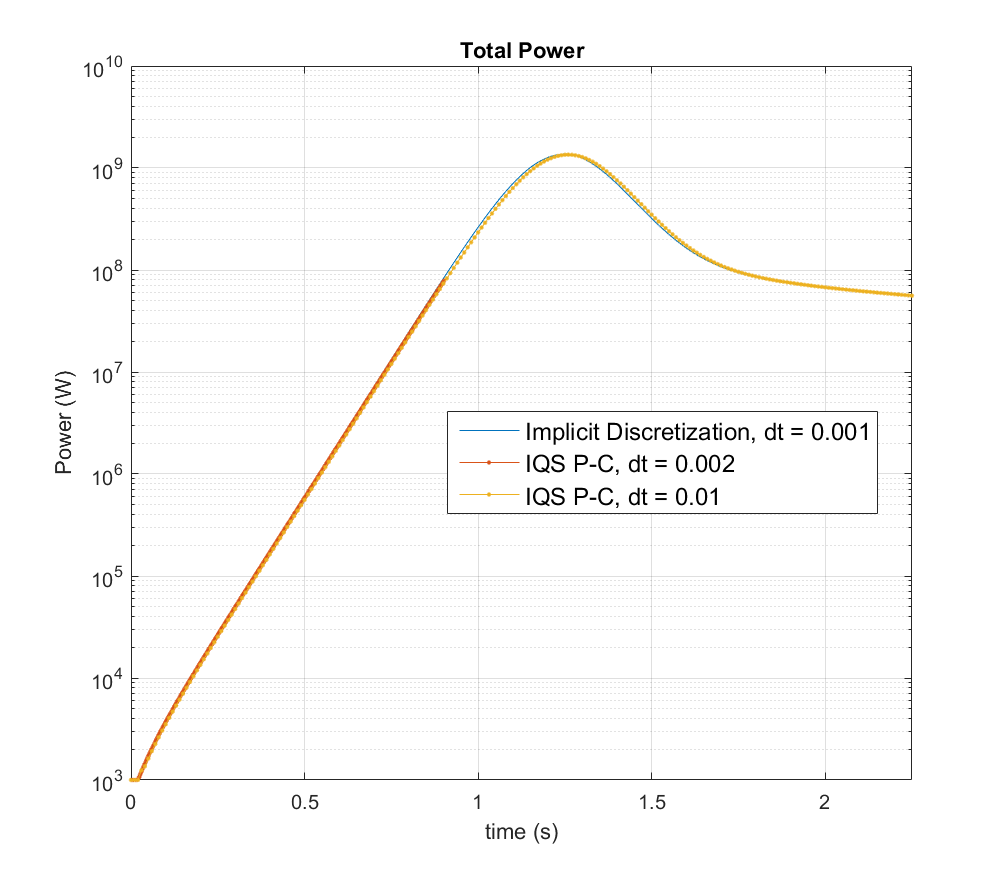
\includegraphics[width=\linewidth]{figures/M8_1.png}
\end{figure}

\column{.6\textwidth}
\begin{figure}
\caption{M8CAL Peak Power Profile}
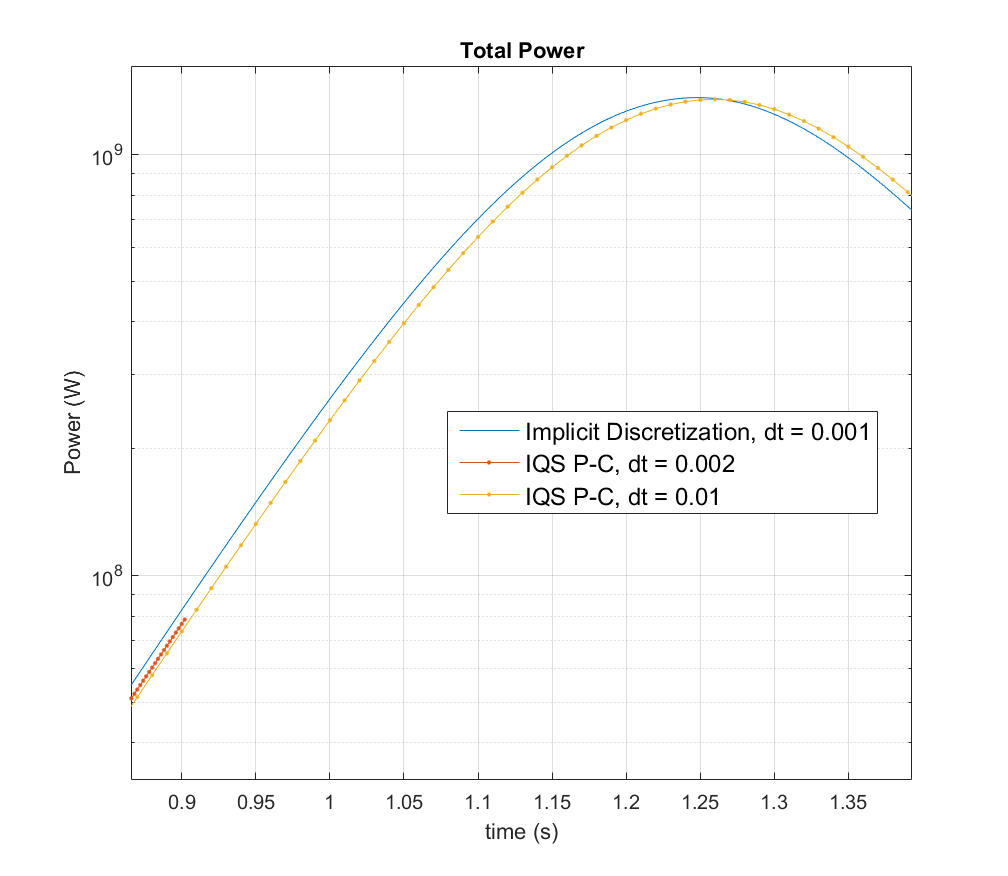
\includegraphics[width=\linewidth]{figures/M8_2.png}
\end{figure}

\end{columns}

\end{frame}
%-------------------------------------------------------------------


%%%%%%%%%%%%%%%%%%%%%%%%%%%%%%%%%%%%%%%%%%%%%%%%%%%%%%%%%%%%%%%%%%%%
%%%%%%%%%%%%%%%%%%%%%%%%%%%%%%%%%%%%%%%%%%%%%%%%%%%%%%%%%%%%%%%%%%%%
\section{Step Doubling}
%%%%%%%%%%%%%%%%%%%%%%%%%%%%%%%%%%%%%%%%%%%%%%%%%%%%%%%%%%%%%%%%%%%%
%%%%%%%%%%%%%%%%%%%%%%%%%%%%%%%%%%%%%%%%%%%%%%%%%%%%%%%%%%%%%%%%%%%%

%-------------------------------------------------------------------
\begin{frame}{Step Doubling}

\tableofcontents[currentsection]

\end{frame}
%-------------------------------------------------------------------

\subsection{Process}

%-------------------------------------------------------------------
\begin{frame}{Step Doubling Solution Process}

\begin{block}{Solution Process with IQS}
\begin{figure}[htpb!]
\centering
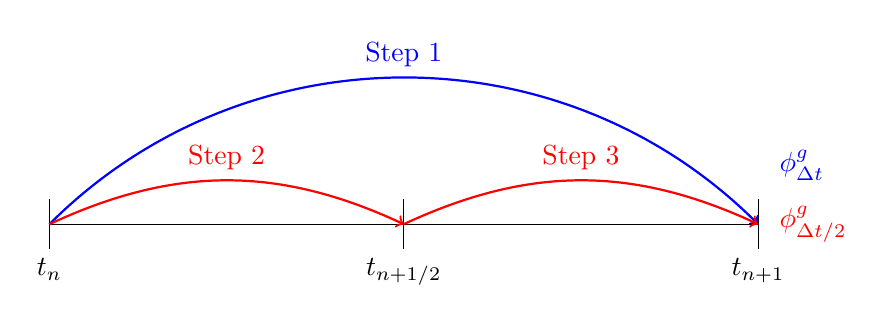
\begin{tikzpicture}[scale=1.5]
\draw[] (0,2) -- (6,2) ;
\foreach \x in  {0,3,6}
\draw[shift={(\x,2)},color=black] (0pt,6pt) -- (0pt,-6pt);
\draw[shift={(0,2)},color=black] (0pt,0pt) -- (0pt,-6pt) node[below] {$t_n$};
\draw[shift={(3,2)},color=black] (0pt,0pt) -- (0pt,-6pt) node[below] {$t_{n+1/2}$};
\draw[shift={(6,2)},color=black] (0pt,0pt) -- (0pt,-6pt) node[below] {$t_{n+1}$};
\draw (0,2) edge[out=45,in=135,->,thick,blue] node[above,sloped] {\tcb{Step 1}} (6,2);
\draw (0,2) edge[out=25,in=155,->,thick,red] node[above,sloped] {\tcr{Step 2}} (3,2);
\draw (3,2) edge[out=25,in=155,->,thick,red] node[above,sloped] {\tcr{Step 3}} (6,2);
\node[anchor=west](shape) at (6.1,2.5) {$\tcb{\phi_{\Delta t}^g}$};
\node[anchor=west](shape) at (6.1,2) {$\tcr{\phi_{\Delta t/2}^g}$};

\end{tikzpicture}
\end{figure}
\be
e_n =\frac{\norm{\sum_{g=1}^G \left(\tcr{\phi^g_{\Delta t/2}} - \tcb{\phi^g_{\Delta t}} \right)}}{\max\left(\norm{\sum_{g=1}^G\tcr{\phi^g_{\Delta t/2}}},\norm{\sum_{g=1}^G\tcb{\phi^g_{\Delta t}}}\right)} 
\qq  \qq 
\Delta t_{new} = S_f \Delta t \left[\frac{e_{tol}}{e_n}\right]^{1/(p+1)}   
\ee

\end{block}
\end{frame}
%-------------------------------------------------------------------

%-------------------------------------------------------------------
\begin{frame}{Step Doubling Solution Process}
\begin{block}{Programming Visualization}
\begin{figure}[!htpb]
\centering
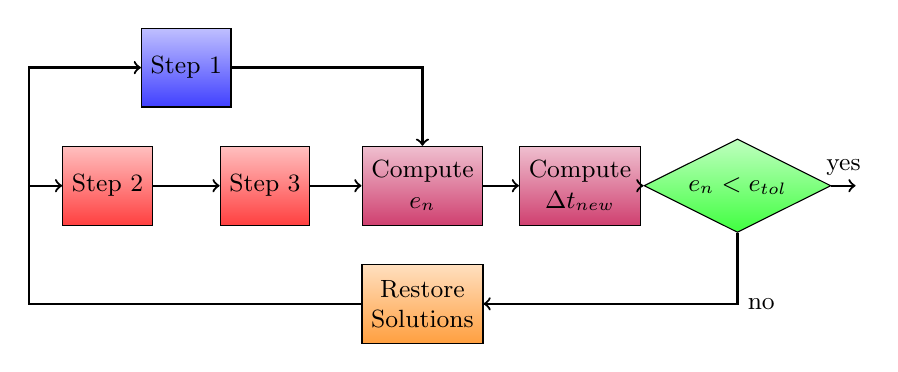
\begin{tikzpicture}[every node/.style = {font=\small},scale=0.5]

\node[blueblock](p1) at (-6,3) {Step 1} ;
\node[redblock](p2) at (-8,0) {Step 2} ;
\node[redblock](p3) at (-4,0) {Step 3} ;
\node[purpleblock](p4) at (0,0) {Compute \\ $e_n$};
\node[purpleblock](p5) at (4,0) {Compute  \\ $\Delta t_{new}$};
\node[greendiamond](p6) at (8,0) {$e_n < e_{tol}$};
\node[orangeblock](p7) at (0,-3) {Restore \\ Solutions};

\draw[->,thick](p1.east) -| (p4.north);
\draw[->,thick](p2.east) -- (p3.west);
\draw[->,thick](p3.east) -- (p4.west);
\draw[->,thick](p4.east) -- (p5.west);
\draw[->,thick](p5.east) -- (p6.west);
\draw[->,thick](p6.south) |- node[right] {no} (p7.east);
\draw[->,thick](p6.east) -- node[above] {yes} (11,0);
\draw[->,thick](p7.west) -| (-10,0) -- (p2.west);
\draw[->,thick](p7.west) -| (-10,0) |- (p1.west);

\end{tikzpicture}
\end{figure}
Each Step undergoes:
\bi
\item Shape evaluation
\item PRKE evaluations
\item Multiphysics evaluations
\item Iterations for convergence of amplitude, shape, and multiphysics
\ei



\end{block}

\end{frame}
%-------------------------------------------------------------------

\subsection{LRA}


%-------------------------------------------------------------------
\begin{frame}{LRA Benchmark}
\begin{columns}

\column{0.6\textwidth}
\begin{figure}
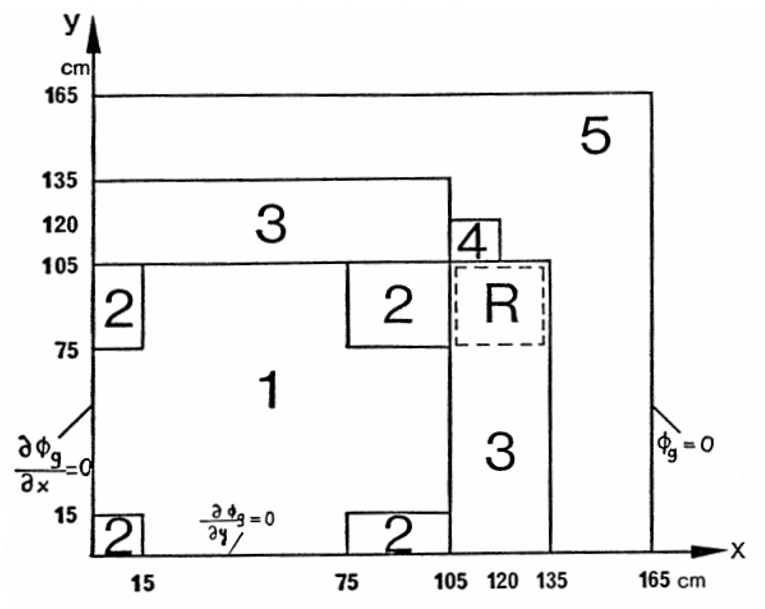
\includegraphics[width=\linewidth]{figures/lra_geom.png}
\end{figure}

\column{0.6\textwidth}
\begin{figure}
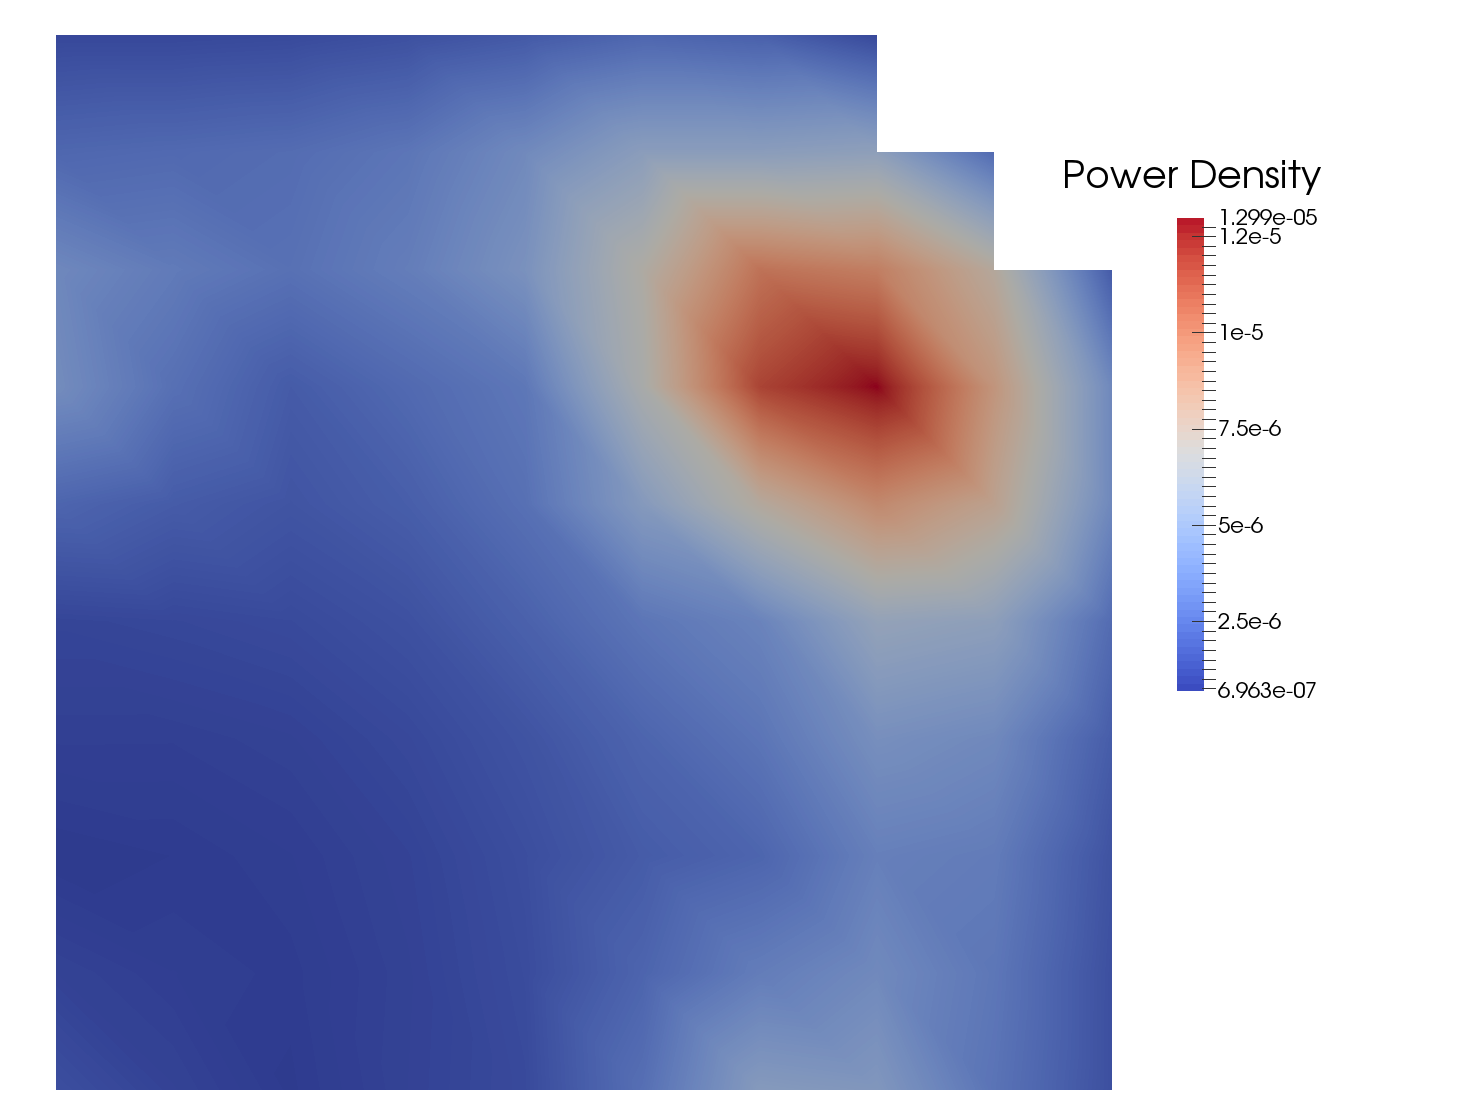
\includegraphics[width=\linewidth]{figures/lra_viz.png}
\end{figure}

\end{columns}
\end{frame}
%-------------------------------------------------------------------

%-------------------------------------------------------------------
\begin{frame}{LRA Results}

\begin{columns}

\column{.6\textwidth}
\begin{figure}
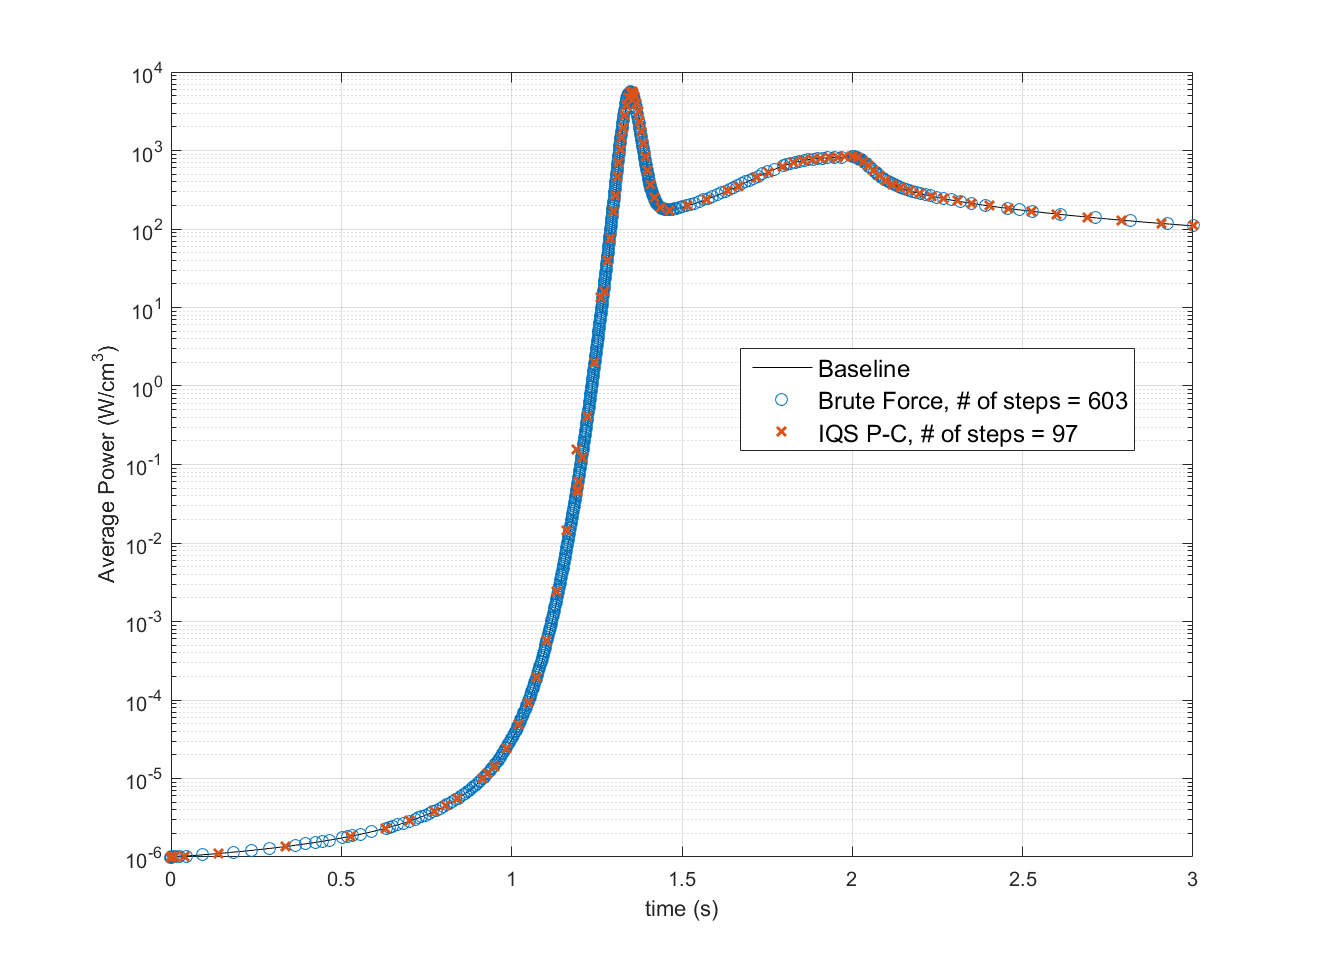
\includegraphics[width=\linewidth]{figures/LRA_DT2.png}
\caption{LRA Power Profile}
\end{figure}

\column{.6\textwidth}
\begin{figure}
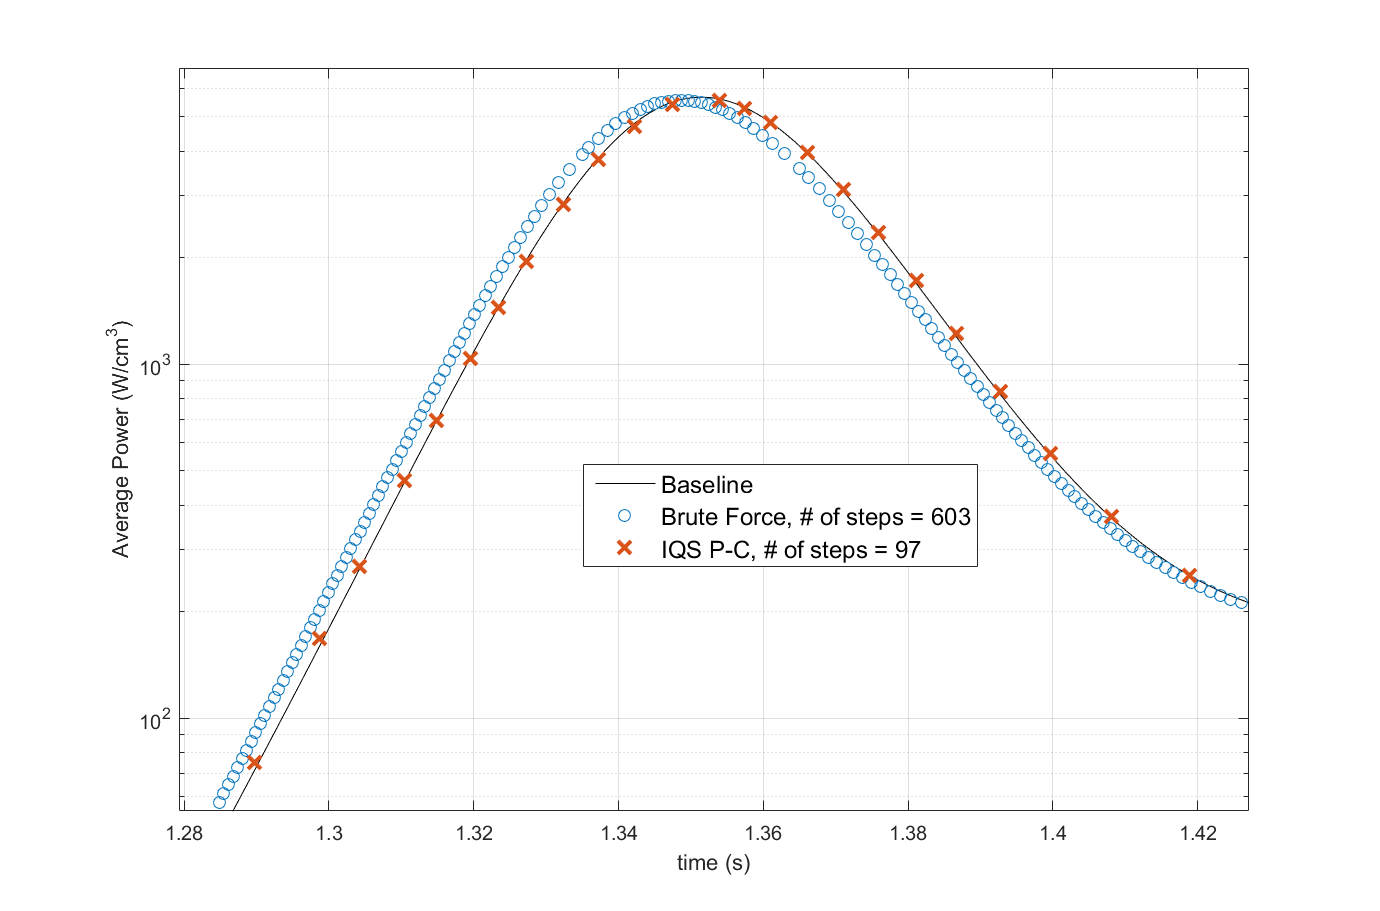
\includegraphics[width=\linewidth]{figures/LRA_DT2_peak.png}
\caption{LRA Peak Power Profile}
\end{figure}

\end{columns}

\vspace{-2mm}

\begin{block}{}
\begin{table}
\begin{center}
\resizebox{\textwidth}{!}{
\begin{tabular}{|l|l|l|l|l|l|l|}
\hline
 & \multicolumn{3}{|c|}{Brute Force} & \multicolumn{3}{|c|}{IQS P-C} \\
\hline
Event & Power (W/cm$^3$) & Error & Steps & Power (W/cm$^3$) & Error & Steps \\
\hline
Max Power & 5567.3 & 0.019454 & 423 & 5568.3 & 0.019274 & 47 \\
End (3 s) & 109.66 & 2.3650e-4 & 603 & 109.65 & 3.0622e-4 & 97 \\
\hline
\end{tabular}}
\end{center}
\end{table}
\end{block}

\end{frame}
%-------------------------------------------------------------------

\subsection{Tran15}

%-------------------------------------------------------------------
\begin{frame}{Tran15 Results}

\begin{columns}

\column{.6\textwidth}
\begin{figure}
\caption{Tran15 Power Profile}
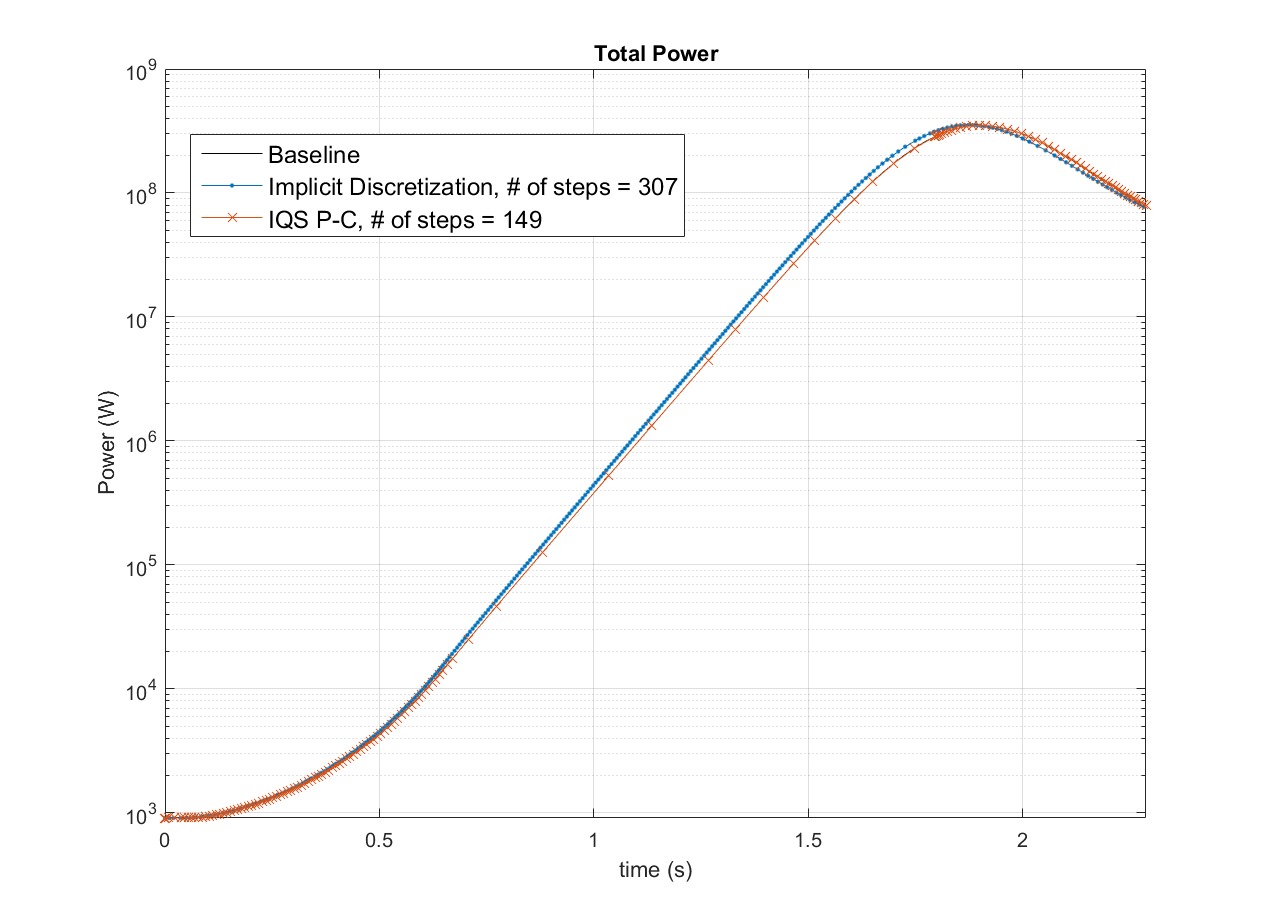
\includegraphics[width=\linewidth]{figures/Tran15_DT2.png}
\end{figure}

\column{.6\textwidth}
\begin{figure}
\caption{Tran15 Peak Power Profile}
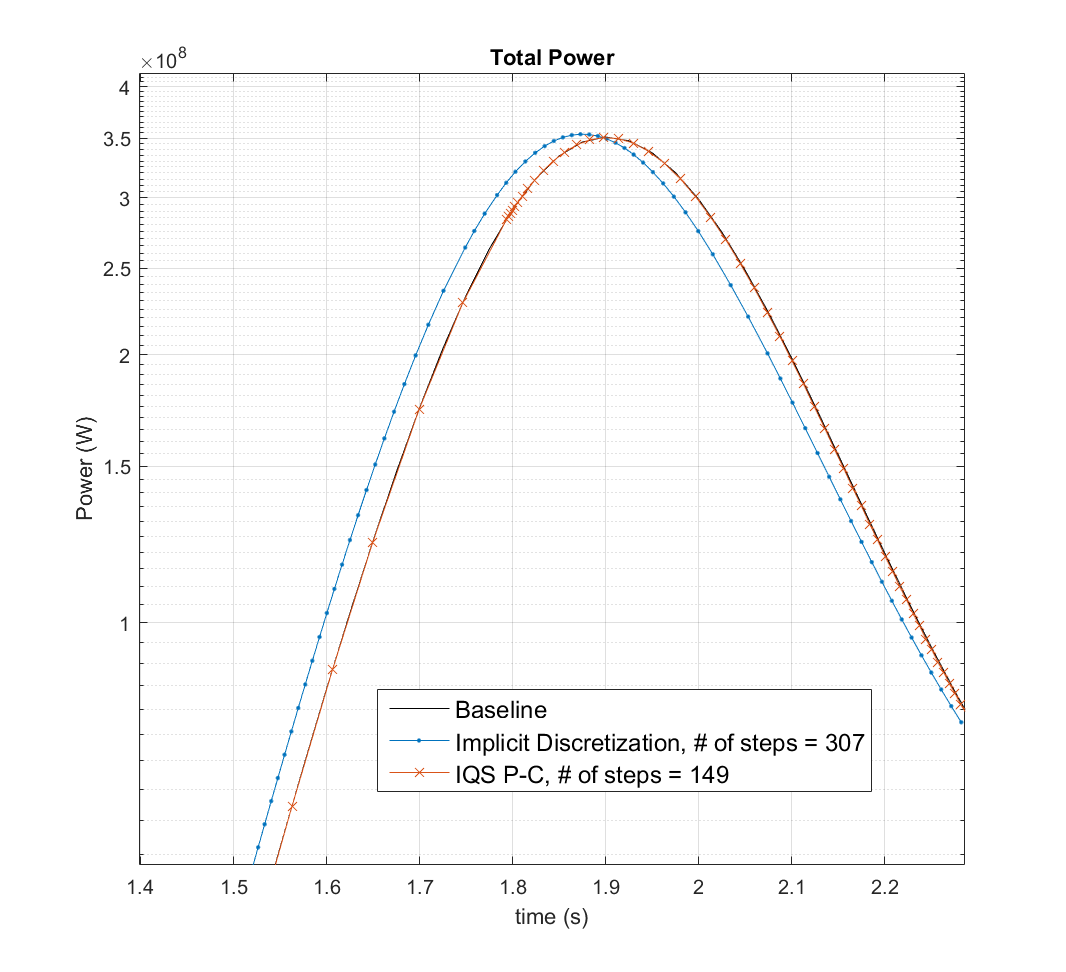
\includegraphics[width=\linewidth]{figures/Tran15_DT2_peak.png}
\end{figure}

\end{columns}

\end{frame}
%-------------------------------------------------------------------



%%%%%%%%%%%%%%%%%%%%%%%%%%%%%%%%%%%%%%%%%%%%%%%%%%%%%%%%%%%%%%%%%%%%
%%%%%%%%%%%%%%%%%%%%%%%%%%%%%%%%%%%%%%%%%%%%%%%%%%%%%%%%%%%%%%%%%%%%
\section{Multiphysics Updates}
%%%%%%%%%%%%%%%%%%%%%%%%%%%%%%%%%%%%%%%%%%%%%%%%%%%%%%%%%%%%%%%%%%%%
%%%%%%%%%%%%%%%%%%%%%%%%%%%%%%%%%%%%%%%%%%%%%%%%%%%%%%%%%%%%%%%%%%%%


%-------------------------------------------------------------------
\begin{frame}{Multiphysics Updates}

\tableofcontents[currentsection]

\end{frame}
%-------------------------------------------------------------------

%-------------------------------------------------------------------
\begin{frame}{Motivation}

\begin{columns}

\column{.6\textwidth}
\begin{figure}
\caption{LRA convergence at $t=1.44s$}
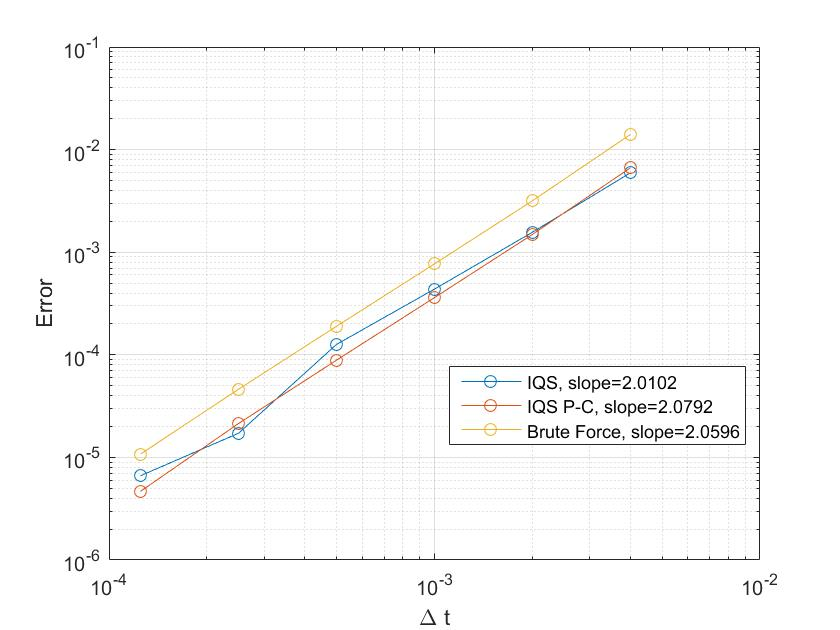
\includegraphics[width=\linewidth]{figures/lra_bad.jpg}
\end{figure}

\column{.6\textwidth}
\begin{figure}
\caption{LRA convergence at $t=1.40s$}
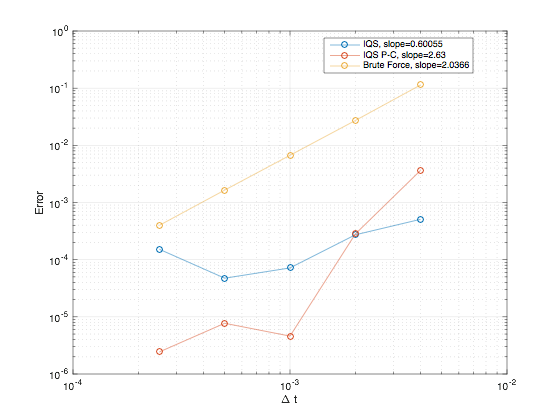
\includegraphics[width=\linewidth]{figures/lra_good.png}
\end{figure}

\end{columns}

\end{frame}
%-------------------------------------------------------------------

\subsection{Process}

%-------------------------------------------------------------------
\begin{frame}{Multiphysics Timescale}

\begin{figure}
\resizebox{\columnwidth}{!}{
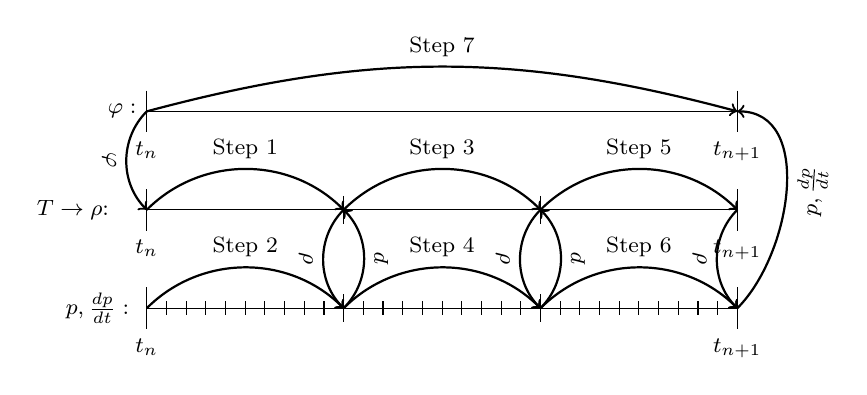
\begin{tikzpicture}[scale=1.25]
\tikzset{font={\footnotesize}}
%Shape
\draw[] (0,2) -- (6,2) ;
\foreach \x in  {0,6}
\draw[shift={(\x,2)},color=black] (0pt,6pt) -- (0pt,-6pt);
\draw[shift={(0,2)},color=black] (0pt,0pt) -- (0pt,-6pt) node[below] {$t_n$};
\draw[shift={(6,2)},color=black] (0pt,0pt) -- (0pt,-6pt) node[below] {$t_{n+1}$};
\node(shape) at (-.25,2) {$\varphi:$};

%Temp/Params
\draw[] (0,1) -- (6,1) ;
\foreach \x in  {0,6}
\draw[shift={(\x,1)},color=black] (0pt,6pt) -- (0pt,-6pt);
\foreach \x in  {2,4}
\draw[shift={(\x,1)},color=black] (0pt,4pt) -- (0pt,-4pt);
\draw[shift={(0,1)},color=black] (0pt,0pt) -- (0pt,-6pt) node[below] {$t_n$};
\draw[shift={(6,1)},color=black] (0pt,0pt) -- (0pt,-6pt) node[below] {$t_{n+1}$};
\node(temp) at (-.75,1) {$T \rightarrow \rho$:};

% PRKE
\draw[] (0,0) -- (6,0) ;
\foreach \x in  {0,6}
\draw[shift={(\x,0)},color=black] (0pt,6pt) -- (0pt,-6pt);
\foreach \x in  {0,2,4,6}
\draw[shift={(\x,0)},color=black] (0pt,4pt) -- (0pt,-4pt);
\foreach \x in  {0,0.2,0.4,0.6,0.8,1,1.2,1.4,1.6,1.8,2,2.2,2.4,2.6,2.8,3,3.2,3.4,3.6,3.8,4,4.2,4.4,4.6,4.8,5,5.2,5.4,5.6,5.8,6}
\draw[shift={(\x,0)},color=black] (0pt,2pt) -- (0pt,-2pt);
\draw[shift={(0,0)},color=black] (0pt,0pt) -- (0pt,-6pt) node[below] {$t_n$};
\draw[shift={(6,0)},color=black] (0pt,0pt) -- (0pt,-6pt) node[below] {$t_{n+1}$};
\node(prke) at (-.5,0) {$p, \frac{dp}{dt}:$};

\draw (0,0) edge[out=45,in=135,->,thick] node[above,sloped] {Step 2} (2,0);
\draw (2,0) edge[out=45,in=135,->,thick] node[above,sloped] {Step 4} (4,0);
\draw (4,0) edge[out=45,in=135,->,thick] node[above,sloped] {Step 6} (6,0);
\draw (0,1) edge[out=45,in=135,->,thick] node[above,sloped] {Step 1} (2,1);
\draw (2,1) edge[out=45,in=135,->,thick] node[above,sloped] {Step 3} (4,1);
\draw (4,1) edge[out=45,in=135,->,thick] node[above,sloped] {Step 5} (6,1);
\draw (0,2) edge[out=15,in=165,->,thick] node[above,sloped] {Step 7} (6,2);

\draw (0,2) edge[out=-135,in=135,->,thick] node[below,sloped] {$\varphi$} (0,1);
\draw (2,1) edge[out=-135,in=135,->,thick] node[below,sloped] {$\rho$} (2,0);
\draw (2,0) edge[out=45,in=-45,->,thick] node[below,sloped] {$p$} (2,1);
\draw (4,1) edge[out=-135,in=135,->,thick] node[below,sloped] {$\rho$} (4,0);
\draw (4,0) edge[out=45,in=-45,->,thick] node[below,sloped] {$p$} (4,1);
\draw (6,1) edge[out=-135,in=135,->,thick] node[below,sloped] {$\rho$} (6,0);
\draw (6,0) edge[out=45,in=0,->,thick] node[below,sloped] {$p, \frac{dp}{dt}$} (6,2);

\end{tikzpicture}
}
\end{figure}

\end{frame}
%-------------------------------------------------------------------

\subsection{LRA}

%-------------------------------------------------------------------
\begin{frame}{LRA with New Timescale}

\begin{columns}

\column{.6\textwidth}
\begin{figure}
\caption{LRA multiphysics updates convergence}
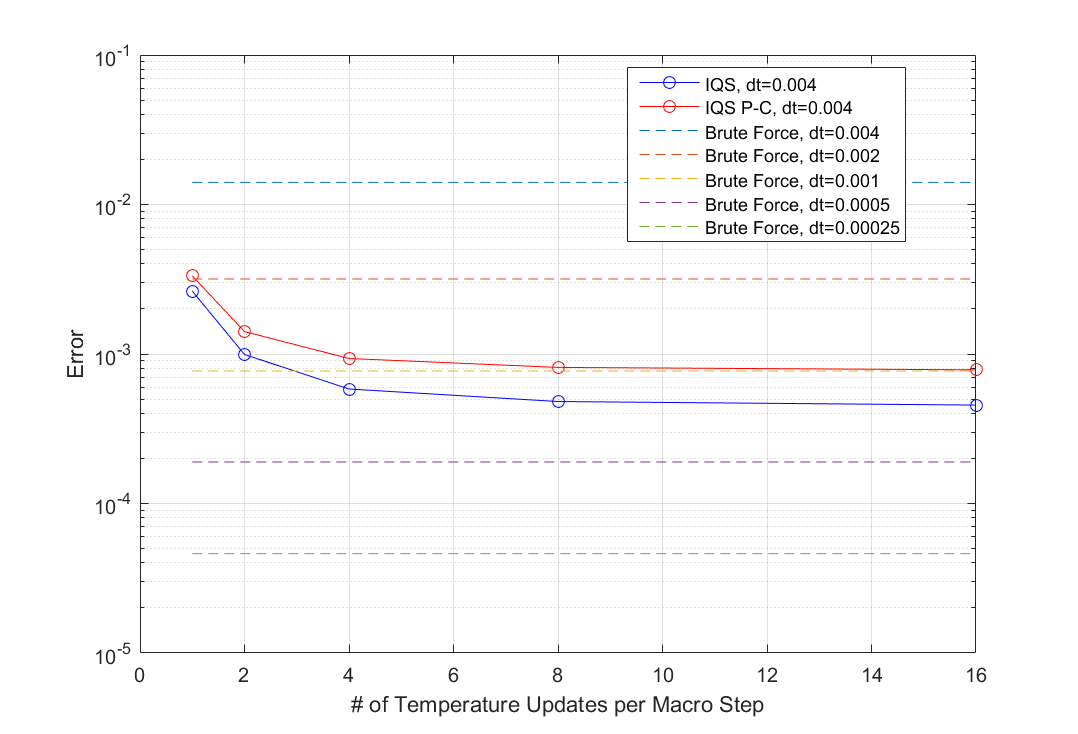
\includegraphics[width=\linewidth]{figures/lra_mp.png}
\end{figure}

\column{.6\textwidth}
\begin{figure}
\caption{LRA convergence at $t=1.44s$}
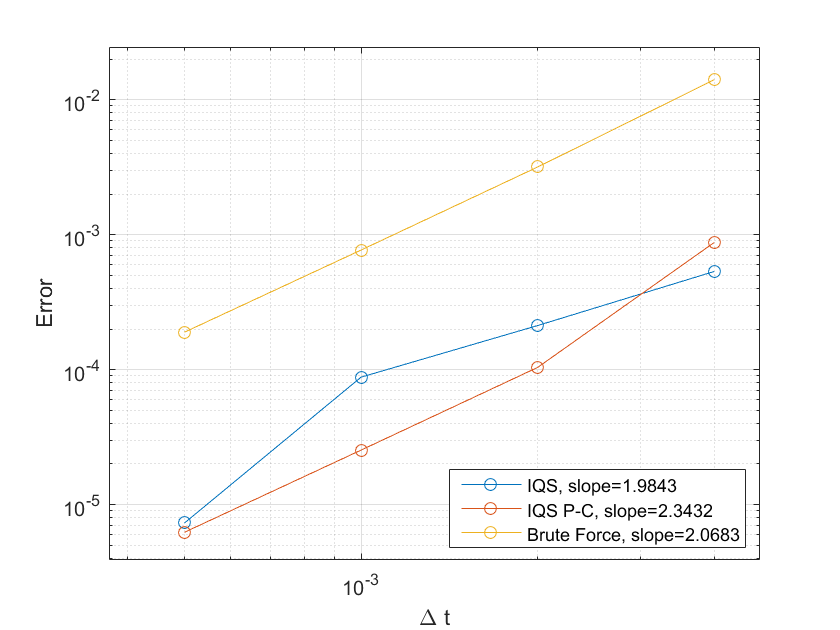
\includegraphics[width=\linewidth]{figures/lra_mp_convergence.png}
\end{figure}

\end{columns}

\end{frame}
%-------------------------------------------------------------------


%%%%%%%%%%%%%%%%%%%%%%%%%%%%%%%%%%%%%%%%%%%%%%%%%%%%%%%%%%%%%%%%%%%%
%%%%%%%%%%%%%%%%%%%%%%%%%%%%%%%%%%%%%%%%%%%%%%%%%%%%%%%%%%%%%%%%%%%%
\section{IQS Refactoring}
%%%%%%%%%%%%%%%%%%%%%%%%%%%%%%%%%%%%%%%%%%%%%%%%%%%%%%%%%%%%%%%%%%%%
%%%%%%%%%%%%%%%%%%%%%%%%%%%%%%%%%%%%%%%%%%%%%%%%%%%%%%%%%%%%%%%%%%%%


%-------------------------------------------------------------------
\begin{frame}{IQS Refactoring}

\tableofcontents[currentsection]

\end{frame}
%-------------------------------------------------------------------

%-------------------------------------------------------------------
\begin{frame}{Executioner, User Object, Postprocessor, Postprocessor, Postprocessor, ...}

\begin{block}{Current Implementation}
\begin{figure}[h]
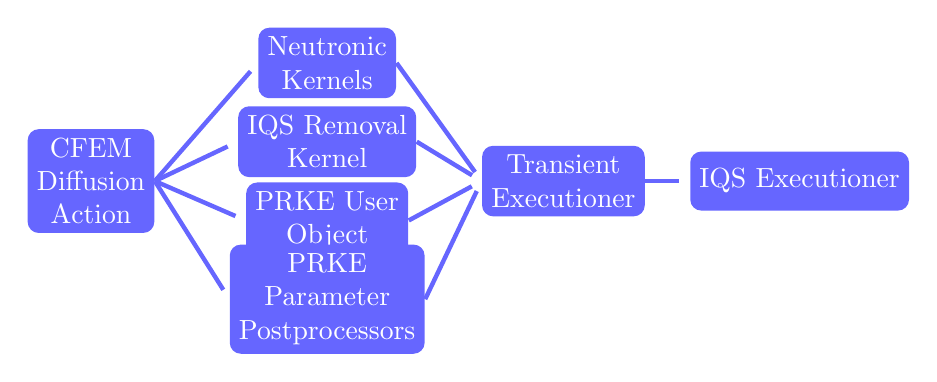
\begin{tikzpicture}[every node/.style = {shape          = rectangle, rounded corners, fill = blue!60, minimum width  = 1.5cm, minimum height = 0.75cm, align= center, text = white},blue edge/.style  = { -, ultra thick, blue!60, shorten >= 4pt}]
\node(0;0) at (-1,0) {CFEM \\ Diffusion \\ Action};
  \node(1;3)  at (2, 1.5) {Neutronic \\ Kernels};   
  \node(1;1)  at (2, 0.5) {IQS Removal \\ Kernel}; 
  \node(1;-1)  at (2,-0.5) {PRKE User \\ Object}; 
  \node(1;-3) at (2,-1.5) {PRKE \\ Parameter \\ Postprocessors}; 
     \node(2;0)  at (5,0) {Transient \\ Executioner};
     	\node(3;0)  at (8,0) {IQS Executioner};
\foreach \j in {-3,-1,1,3}
  { \draw[blue edge] (0;0.east) -- (1;\j.west); }
\foreach \j in {-3,-1,1,3}
  { \draw[blue edge] (1;\j.east) -- (2;0.west);} 
\draw[blue edge] (2;0.east) -- (3;0.west);         
\end{tikzpicture}
%\caption{CFEM Diffusion Action Process Diagram}   
\label{Action}
\end{figure}
\end{block}

\begin{block}{What's Wrong?}
\bi
\item Multitudinous postprocessors
\item Weakly defined $\rho$ with \texttt{save\_in}
\item Lots of duplicate code between Transient and IQS executioner 
\ei
\end{block}

\end{frame}
%-------------------------------------------------------------------

%-------------------------------------------------------------------
\begin{frame}{User Objects}

\begin{block}{Proposed Implementation}
\begin{figure}[h]
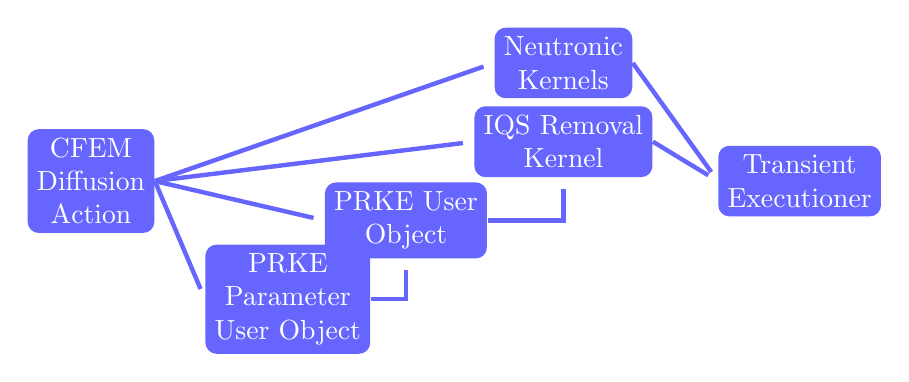
\begin{tikzpicture}[every node/.style = {shape          = rectangle, rounded corners, fill = blue!60, minimum width  = 1.5cm, minimum height = 0.75cm, align= center, text = white},blue edge/.style  = { -, ultra thick, blue!60, shorten >= 4pt}]
\node(0;0) at (-1,0) {CFEM \\ Diffusion \\ Action};
  \node(1;3)  at (5, 1.5) {Neutronic \\ Kernels};   
  \node(1;1)  at (5, 0.5) {IQS Removal \\ Kernel}; 
  \node(1;-1)  at (3,-0.5) {PRKE User \\ Object}; 
  \node(1;-3) at (1.5,-1.5) {PRKE \\ Parameter \\ User Object}; 
  \node(2;0)  at (8,0) {Transient \\ Executioner};

\foreach \j in {-3,-1,1,3}
  { \draw[blue edge] (0;0.east) -- (1;\j.west); }
\foreach \j in {1,3}
  { \draw[blue edge] (1;\j.east) -- (2;0.west);} 
\draw[blue edge](1;-1.east) -| (1;1.south);
\draw[blue edge](1;-3.east) -| (1;-1.south);

  

\end{tikzpicture}
\label{Action}
\end{figure}
\end{block}

\begin{block}{What's Good?}
\bi
\item Less files and duplicate code
\item IQS iteration at PFJNK level (Picard currently)
\item Easier integration of other transport systems
\ei
\end{block}

\end{frame}
%-------------------------------------------------------------------




%%%%%%%%%%%%%%%%%%%%%%%%%%%%%%%%%%%%%%%%%%%%%%%%%%%%%%%%%%%%%%%%%%%%%
%%%%%%%%%%%%%%%%%%%%%%%%%%%%%%%%%%%%%%%%%%%%%%%%%%%%%%%%%%%%%%%%%%%%%
\section{Wrap-up}
%%%%%%%%%%%%%%%%%%%%%%%%%%%%%%%%%%%%%%%%%%%%%%%%%%%%%%%%%%%%%%%%%%%%%
%%%%%%%%%%%%%%%%%%%%%%%%%%%%%%%%%%%%%%%%%%%%%%%%%%%%%%%%%%%%%%%%%%%%%

%-------------------------------------------------------------------
\begin{frame}{Wrap-up}

\tableofcontents[currentsection]

\end{frame}
%-------------------------------------------------------------------


%-------------------------------------------------------------------
\begin{frame}{IQS Update}

\begin{block}{Honey-Done List}
\bi
\item Initial IQS implementation to TREAT examples
\item IQS testing with step doubling
\item Initial thoughts on IQS multiphysics 
\ei
\end{block}

\begin{block}{Honey-Do List}
\bi 
\item Waiting on MOOSE to finish refactoring time steppers so Rattlesnake can have step doubling
\item IQS multiphysics with multi-apps in mind
\item Refactor IQS executioner to user object
\ei
\end{block}

\end{frame}
%-------------------------------------------------------------------

%-------------------------------------------------------------------
\begin{frame}{Questions about IQS?}

\begin{block}{Thank you}
\begin{itemize}
\item Yaqi Wang (INL, Rattlesnake lead)
\item Mark DeHart (INL, TREAT M\&S lead)
\item NEAMS
\end{itemize}
\end{block}

\begin{block}{}
\begin{figure}
	What people think when I say I work on TREAT \\
	\centering
	
\includegraphics[scale=0.35]{figures/cookie_monster.jpg}
\end{figure}
\end{block}


\end{frame}
%-------------------------------------------------------------------

%-------------------------------------------------------------------
\begin{frame}{Uh oh ... More? Performance Analysis on Tran15}

\begin{block}{Computing Time}
96 CPUs, 65 Time Steps
\begin{table}
\begin{center}
\resizebox{\textwidth}{!}{
\begin{tabular}{|l|l|l|l|}
\hline
Process & Time (hr) & Time per Step (sec) & \% of Time \\
\hline
\texttt{compute\_residual()} & 6.87 & 381 & 36\% \\
\texttt{solve()} & 6.66 & 369 & 35\% \\
\texttt{update\_aux\_vars\_elemental() } & 5.01 & 277 & 27\% \\
Total & 18.85 & 1044 & 100\% \\
\hline
\end{tabular}}
\end{center}
\end{table}
\end{block}

\begin{block}{Number of Iterations}
\begin{itemize}
\item Number of Steps: 65
\item Number of Nonlinear iterations per step: 3
\item Number of Linear iterations per step: 180
\item Number of Linear iterations per Nonlinear iteration: 60
\end{itemize}
\end{block}


\end{frame}
%-------------------------------------------------------------------

%-------------------------------------------------------------------
\begin{frame}{Preconditioning}

\vspace{-2mm}

\begin{block}{Jacobian Sparsity}
\begin{figure}
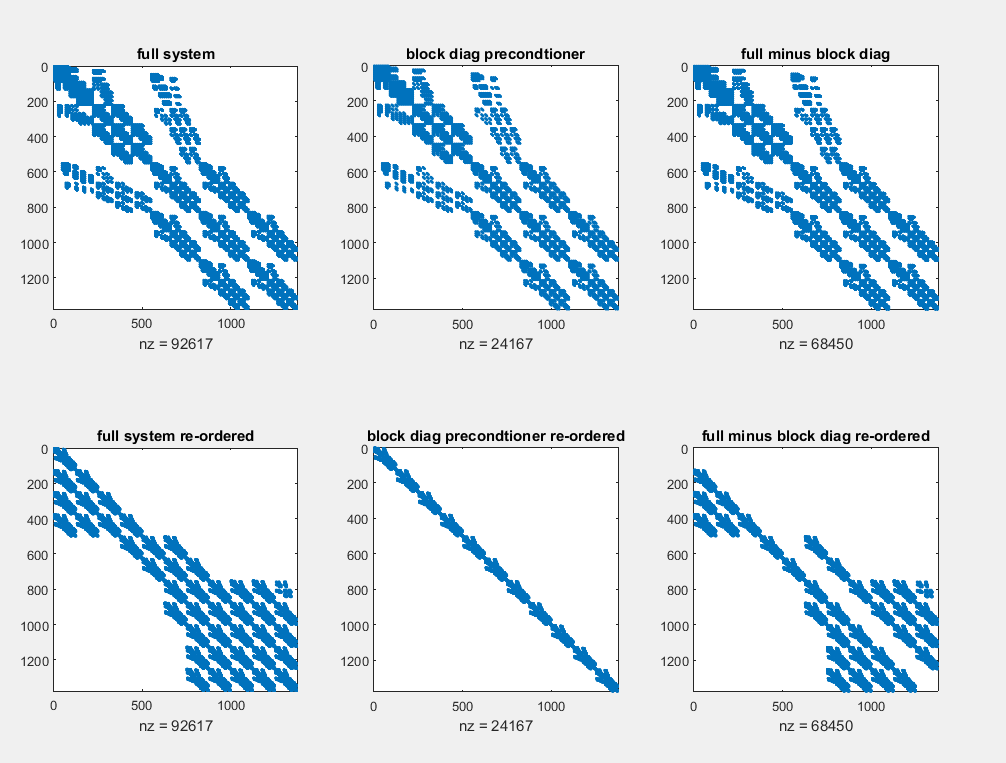
\includegraphics[height=2.75in]{figures/jacobian.png}
\end{figure}
\end{block}


\end{frame}
%-------------------------------------------------------------------

%-------------------------------------------------------------------
\begin{frame}{Preconditioning}

\vspace{-2mm}

\begin{block}{GMRES Convergence}
\begin{figure}
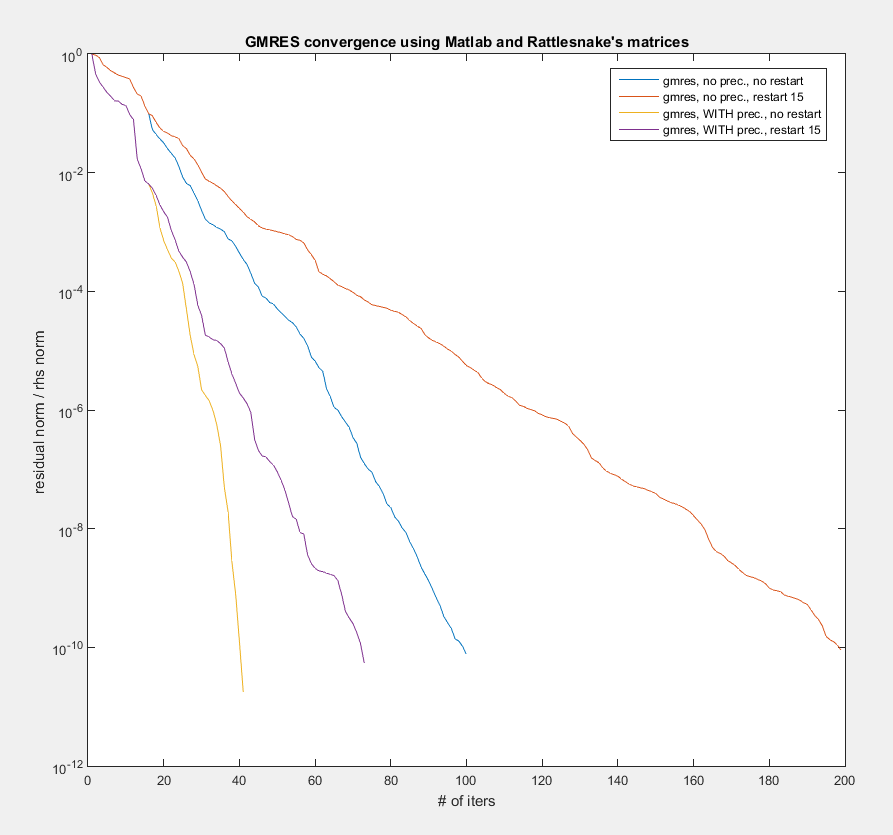
\includegraphics[height=2.75in]{figures/gmres_convergence.png}
\end{figure}
\end{block}


\end{frame}
%-------------------------------------------------------------------

%-------------------------------------------------------------------
\begin{frame}{Whew!}
\centering

\includegraphics[scale=0.2]{figures/question_mark.jpg}

\end{frame}



%************************************************

\end{document}